\documentclass[main]{subfiles}
\begin{document}
%@@@@@@@@@@@@@@@@@@@@@@@@@@@@@@
% summarizes lecture 4
% author: Joachim Ott
\section{Source Follower}
%Joachim
The source follower
\begin{itemize}
\item Transforms a weakly-driven voltage signal into a more strongly-driven voltage signal
\item Is a two transistor circuit consisting of two MOSFET in series
\item Consists of a fixed current source that is connected to the source of another MOSFET in saturation 
\item Linearly transforms a voltage $V_{in}$ at a high impedance input terminal $M_1$ into a voltage at a lower impedance output terminal $V_{out}$
\subitem M1 source is equal to $V_{out}$
\subitem $V_{out}$ is able to drive larger loads
\end{itemize}

\begin{figure}[htbp]
  \centering
  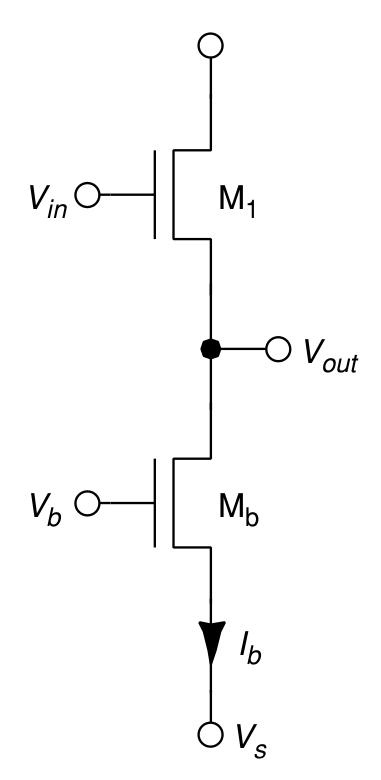
\includegraphics[scale=1]{pics/source-follower.png}
  \caption{Source Follower Circuit \cite{book:VLSI}}
  \label{fig:Source_Follower_Structure}
\end{figure}

\subsection{Proper Operation Requirements}
Saturation of the biasing transistor: $V_{out} > V_s + 4U_T$\\
that is $V_{in} > K_{n}^{-1}(\kappa_b V_b + 4U_T)$

\subsection{Subthreshold Operation}
In subthreshold, the output voltage changes according to:
\begin{equation}
V_{out}=\kappa_n V_{in} - U_T log(\frac{I_b}{I_{n0}}) = \kappa_n V_{in} - \kappa_b V_b + V_s
\end{equation}
\begin{center}
$\kappa_b$ is the subthreshold slope factor of $M_b$\\
\end{center}
$V_{out}$ is linearly related to $V_{in}$
\begin{itemize}[label={}]
\item $1 >\kappa_n >0$
\item $V_{out}$ has a fixed offset that depends on bias current $I_b$
\end{itemize}

\subsection{Gain}
$V_{out}$ follows $V_{in}$ with gain of $K_n$\\
Important: $K_n$ is not constant due to the body effect of $M_n$

%Joachim End
\end{document}